\section{Results, Generalizations and Limitations}

\subsection{Results}

The circuit obtained in the previous section can be applied to a system o 4 qubits several times to perform a random walk. 
Fig. 2 shows the results of a 100 steps random walks, obtained by apply the circuit 100 times. 

\begin{figure}[h!]
    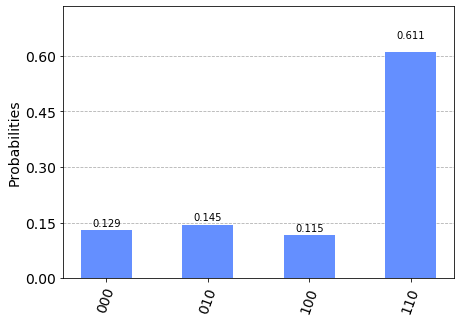
\includegraphics[scale=0.4]{img/100_steps_walk.png}
    \caption{results of a 100 step random walk}
    \centering
\end{figure}

As we can notice in the picture the probailities of find the walker in a given position are 
quite asymmetrical and also odd numbers have zero probability of being measured, this is due to 
the Hadamard coin, in fact, differently from classical, we can 
see a true randomness behavior different from a Gaussian distribution that we will obaserve in a 
classical random walk. This asymmetrical behavior can be modified changing the initial state or 
changing the coin, a more formal description of this behavior is showed in \cite{6812670}.

\subsection{Generalizations}

The example presented is just an application to cyclic graph, also the 3 main component presented, the walker, 
the coin and the shift operator are quite generic. This method in fact can fit different type of problems and graph.
Starting from the coin there are many others operator that we can use, which are symmetrical, other examples are the 
Groover coin or a Balanced coins that get rid of this asymmetrical behavior of the Hadamard coin. For more details
about this coin an introductory summary can be found in \cite{Kempe_2003}, but there are also Quantum walks without
the coin, as it is mentioned in \cite{6812670}.

% generalization for the graphs

The interesting thing is that the example presented can be adpted to a variety of other graphs, for instance we can
build a circuit able to perform a quantum walks also for completed graphs, hypercube, glued trees and others. 
Obviusly, changing the graph, the circuit needs to be adapted but the idea remains the same. A very usefull 
references that shows circuits for the type of graphs mentioned is \cite{douglas2007efficient}

% multi controlled toffoli remark

An important remark concern the total qubits needed, as mentioned in the previous section if
the number of qubits is greather than 2 we need to use multi toffoli gate, this gates can be 
obtained by combining several toffoli gates, with the help of some ancillary qubits, those 
ancillary qubits are needed just to construct the multi controlled toffoli. In Fig. 3 below
is showed how to implement a multi controlled toffoli gates with 5 controls qubits, 
this image is taken from \cite{nielsen_chuang_2010}. In general following this procedure
we need a number of ancillary equals to controls qubits - 1.

\begin{figure}[h!]
    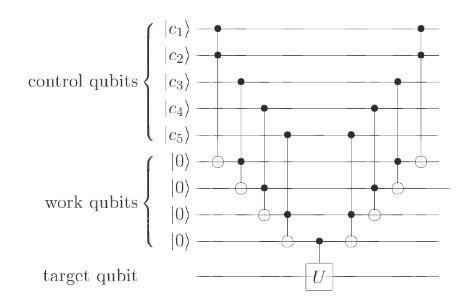
\includegraphics[scale=0.5]{img/ancillary.jpg}
    \caption{Practical representation of multi toffoli gate}
    \centering
\end{figure}

The number of ancillary qubits inpacts also in the efficiency of the circuit. In the next
section will be provided a more formal description of efficiency.

\subsection{Limitations}

The method presented, as we just said, can be generalized to other types of graphs but unfortunately is limited to undirected graphs
without weights, since various application require weighted and/or directed graphs we need something more generic. In the next chapter
is showed a method that can achieve quantum walks also for undirected and weighted graphs. Before presenting this method, we need a 
brief introduction to Markow Chain, using the Markow Chain representation of the graph we can reduce the limitations and work with 
directed and weighted graphs.